\section{Dynamic Scheduler Results Under Fixed and Variable Load}
\label{sec:dynamicresults}
This section reports the two prospectively frozen reviewer campaigns and the two diagnostic protocols. R1 stresses a fixed-load confidence cascade; R2 stresses a load- and prevalence-varying factorial with an explicit one-second deadline SLO. R3 is a predeclared stop and R4 is a validation-only calibration diagnostic. Together they measure when conditional selection adds value and when it does not.

\subsection{R1: Fixed-Rate Confidence Cascade}
Table~\ref{tab:r1} reports ten new matched blocks at 100 rows/s. The fixed cascade escalates 1.34\% of rows and raises F1 by 1.347~pp over Static-LightLR while spending +7.952~J with 95\% CI $[5.897,\,10.007]$~J. Its raw mean-power difference is +15.917~mW $[11.798,\,20.035]$, whereas the preceding-idle adjustment gives +13.635~mW $[-1.515,\,28.784]$: environmental drift therefore weakens the power attribution but not the raw-energy result. Cascade F1 (0.98391) matches Static-MedRF (0.98386) within a few $10^{-5}$, at 0.279~pp lower recall and 0.156~pp lower FPR.

\begin{table*}[t]
\centering\footnotesize
\caption{R1 fixed-rate physical results; means over ten paired blocks. Adjusted power subtracts the immediately preceding idle. Escalation is the fraction sent from LightLR to MedRF.}
\label{tab:r1}
\setlength{\tabcolsep}{4.0pt}
\begin{tabular}{lrrrrrrr}\toprule
Method & Energy (J) & Power (W) & Adjusted (mW) & F1 & Recall (\%) & FPR (\%) & Escalation (\%)\\\midrule
\tableinput{tables/r1_revision_rows}
\bottomrule\end{tabular}
\end{table*}

\subsubsection*{Cascade cost is a call-granularity phenomenon, not a bound}
The apparently disproportionate cascade latency at a 1.34\% escalation rate is explained by call granularity. The frozen source performs \emph{one} MedRF call per escalation-active window on the deferred sub-batch, not one MedRF call per deferred row. Although only 1.3388\% of the 500{,}000 rows are deferred, they land in 3{,}338 of 5{,}000 windows (66.76\%), with a mean of only 2.01 deferred rows per active window. No-escalation windows average 1.636~ms; any-escalation windows average 31.884~ms, close to the cost of a single MedRF batch call regardless of sub-batch size; the overall mean is 21.830~ms. This is an operating-point description, not a general bound: an optimized batched cascade with wider windows or amortized MedRF calls would show a different profile. What the measurement establishes is that reporting only the escalation \emph{fraction} would be misleading; escalation \emph{prevalence across windows} is the operational cost driver.

\subsection{R2: Variable-Load Factorial and DeadlineGuard}
R2 is the campaign in which conditional selection can, in principle, demonstrate adaptive value: every 500-second run visits each of the nine load-by-prevalence cells exactly once, followed by a 50-second recovery cell. All controllers see causal telemetry only; no method sees the factorial cell identity. Table~\ref{tab:r2} reports the six-method means; Table~\ref{tab:r2pairs} lists the two paired contrasts we treat as headline endpoints.

\begin{table*}[t]
\centering\footnotesize
\caption{R2 variable-load results over ten paired blocks. Energy is mean$\pm$SD across runs; deadline miss is the fraction of one-second windows missing the service deadline; completion p95 is the 95th-percentile window completion latency.}
\label{tab:r2}
\setlength{\tabcolsep}{3.1pt}
\begin{tabular}{lrrrrrrr}\toprule
Method & Energy (J) & Power (W) & F1 & Recall (\%) & FPR (\%) & Miss (\%) & Completion p95 (s)\\\midrule
\tableinput{tables/r2_revision_rows}
\bottomrule\end{tabular}
\end{table*}

\begin{table}[t]
\centering\scriptsize
\caption{Headline R2 paired contrasts, $n=10$ blocks. $\Delta E$ is first-minus-second method; detection and deadline changes are percentage points.}
\label{tab:r2pairs}
\resizebox{\columnwidth}{!}{%
\begin{tabular}{lrrrr}\toprule
Contrast & $\Delta E$ (J), 95\% CI & $\Delta$F1 & $\Delta$Miss & sign-flip $p$\\\midrule
\tableinput{tables/r2_key_paired_rows}
\bottomrule\end{tabular}}
\end{table}

\subsubsection*{DeadlineGuard: causal switching adds measurable value}
DeadlineGuard executes MedRF in 3{,}500 and LightLR in 1{,}500 of its 5{,}000 windows and records a mean 5.3 switches per run. Against Static-MedRF, it uses 43.714~J less per run (95\% paired CI 41.418--46.010~J), a 2.98\% reduction relative to the 1{,}468.1-J Static-MedRF mean, while cutting the deadline-miss rate by 10.24~pp to zero. The trade-off is 1.373~pp lower F1 and 2.853~pp lower recall. All ten energy differences share sign (exact sign-flip $p=0.00195$). This is the campaign's positive result: a simple causal rule with a single binary observable achieves measurable energy savings and eliminates the SLO violations under variable load, an outcome that neither learned selector reproduces.

Against Static-LightLR, DeadlineGuard trades +7.550~J $[5.033,\,10.068]$ for a +0.06-pp F1 gain and preserves zero deadline misses. This second contrast is deliberately less dramatic: Static-LightLR is already feasible under the deadline SLO at 4{,}000 rows/s because its inference is fast; DeadlineGuard buys back a small detection-quality gap by escalating to MedRF only where that gap matters. The comparison of the two contrasts is the design lesson: DeadlineGuard is not universally optimal; it is optimal against the high-security static baseline that becomes infeasible at the deadline, and moderate against the low-security static baseline that remains feasible.

\subsubsection*{The learned selectors fail to adapt under variable load}
Frozen DQN remains LightLR in all 5{,}000 windows and reproduces the LightLR detection endpoints. Frozen Tabular-Q, in contrast, reaches new load-related states never visited during training; the zero-initialized Q rows are tied, \texttt{np.argmax} returns the first maximum, and TinyDT is action index zero. The registry labels this ``fallback'' but the frozen source contains no separate exception branch: the R2 outcome is the hardware realization of the off-support tie behavior already visible in the 314/324-state TinyDT greedy map of the primary Q table. The resulting run-level F1 is 0.7434 and FPR is 67.76\%. This is a directly transferable safety risk of sparse discrete controllers whose default action ordering is not itself audited.

\subsubsection*{Heterogeneous variance and preceding-idle drift}
R2 raw energy is heterogeneous across methods. For DQN versus Static-LightLR, all ten raw block differences are positive (median +5.72~J; exact sign-flip $p=0.00195$), but a single Block-4 excursion is +392.0~J. That block's preceding idle is 3.919~W with a 49.2~$^{\circ}$C maximum temperature, unlike the other DQN blocks. The excursion inflates the SD of paired differences to 122.2~J and expands the Student-$t$ interval to $[-43.2,\,131.7]$~J. Preceding-idle adjustment does not resolve the DQN--LightLR contrast. We therefore retain both the consistent raw direction and the unstable magnitude and \emph{do not} claim a controller-power attribution, because R3 was not executed. This is exactly the sort of finding for which our protocol requires raw and drift-adjusted endpoints to be reported side by side.

\begin{figure*}[!t]
\centering
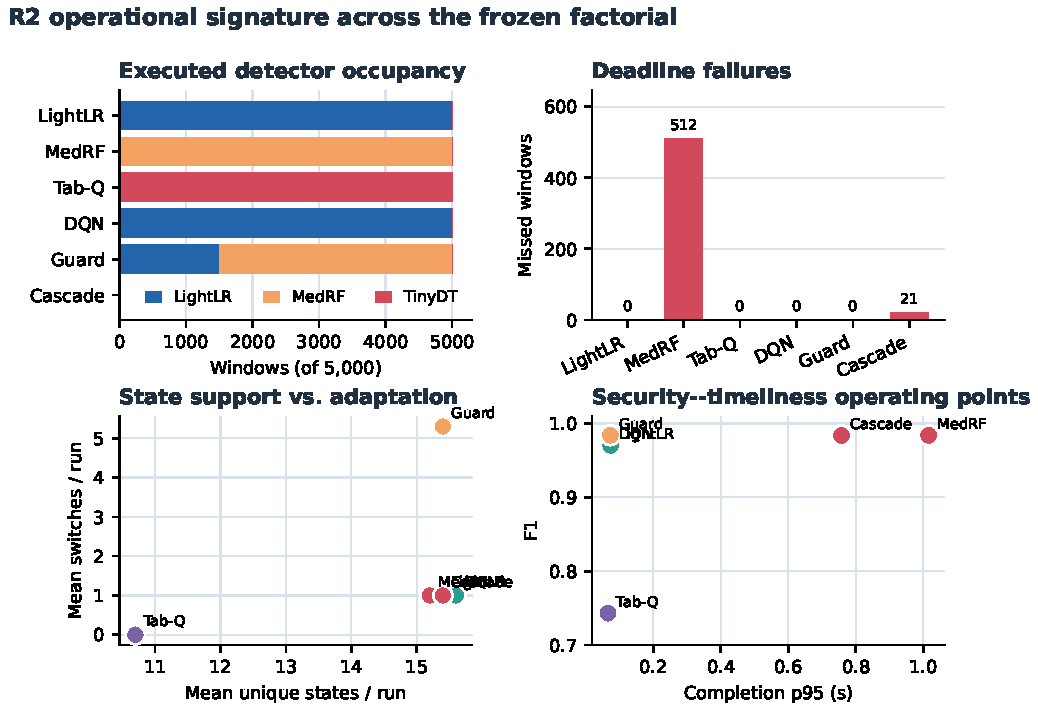
\includegraphics[width=.94\textwidth]{figures/r2_operational_dashboard.pdf}
\caption{R2 operational dashboard: realized detector occupancy, deadline misses, state support and switching, and security--timeliness operating points across the frozen 60-run factorial. DeadlineGuard is the single method with true load-conditioned switching and zero deadline misses; Tabular-Q's TinyDT collapse under new load states is visible in the occupancy panel.}
\label{fig:r2dashboard}
\end{figure*}

\subsection{R3: Protocol-Preserving Stop}
R3 predeclared controller-only physical power over four ``original observed-support states'' for isolated attribution. The frozen artifact exposes eight such states and supplies no outcome-independent rule for selecting four. Choosing four \emph{after the fact} would allow controller-power reporting to be driven by known R2 results, so the campaign stopped before measurement per the predeclared stop rule. No controller-only joule value is claimed. Reporting the stop rather than filling it silently preserves the integrity of the pairwise DQN--LightLR contrast above, which is why the DQN R2 magnitude is deliberately left as unresolved.

\subsection{R4: Threshold Calibration Diagnostic}
R4 selects a TinyDT threshold on validation by maximum balanced accuracy (highest-threshold tie-break), hashes it, and applies it \emph{once} to test. Table~\ref{tab:r4} contrasts the frozen primary threshold with the validation-selected diagnostic.

\begin{table}[t]
\centering\scriptsize
\caption{TON-IoT TinyDT test: fixed primary versus post-hoc validation-selected threshold. The diagnostic does not replace the primary threshold; it isolates calibration sensitivity as an explanation for the primary failure.}
\label{tab:r4}
\setlength{\tabcolsep}{2.1pt}
\resizebox{\columnwidth}{!}{%
\begin{tabular}{lrrrrrrrrr}\toprule
Result & $\tau$ & TN & FP & FN & TP & F1 & Rec. & FPR & BA\\\midrule
\tableinput{tables/r4_threshold_rows}
\bottomrule\end{tabular}}
\end{table}

The diagnostic yields F1 0.9698, FPR 1.82\%, recall 99.61\%, BA 0.9889, and AUROC 0.9906. Recall changes by only 0.15~pp, so the primary failure at threshold 0.5 is substantially calibration-sensitive rather than a symptom of missing ranking information. Two consequences follow. First, TinyDT is not rehabilitated for the frozen physical campaigns: every classifier and scheduler artifact in those campaigns was fixed at threshold 0.5, and no post-hoc threshold can retroactively undo the unsafe TinyDT actions that Tabular-Q emitted under R2. Second, calibration governance---validation-only threshold selection with a hashed freeze before test---is a deployable practice that we recommend for any operational IDS pipeline that includes a TinyDT-class detector.
